\documentclass[conference]{IEEEtran}
\IEEEoverridecommandlockouts

\usepackage{cite}
\usepackage{amsmath,amssymb,amsfonts}
\usepackage{graphicx}
\usepackage{textcomp}
\usepackage{xcolor}
\usepackage{listings}
\usepackage{booktabs}
\usepackage{array}
\usepackage{url}
\usepackage{multirow}
\usepackage{microtype}
\usepackage{float}
\usepackage{tikz}
\usetikzlibrary{arrows.meta,positioning}

\graphicspath{{../}}

% ── Code listing style ───────────────────────────────────────────────────────
\lstdefinestyle{tscode}{
  basicstyle=\ttfamily\scriptsize,
  keywordstyle=\color{blue!70!black},
  commentstyle=\color{green!50!black},
  stringstyle=\color{orange!70!black},
  breaklines=true,
  showstringspaces=false,
  tabsize=2,
  frame=single,
  framesep=2pt,
  xleftmargin=4pt,
  xrightmargin=4pt,
  columns=flexible,
  keepspaces=true,
  morekeywords={interface,const,let,async,await,export,
                import,type,from,as,of,extends,implements,
                function,return,new,true,false,null,undefined}
}
\lstset{style=tscode}

% Convenience macro for inline code (no underscores — use \lstinline for those)
\newcommand{\code}[1]{\texttt{\small #1}}

% ─────────────────────────────────────────────────────────────────────────────
\begin{document}

\title{Measuring the Cost of State: A Controlled Benchmark of Seven
React State Management Libraries in Table-Based Dashboards}

\author{\IEEEauthorblockN{Ihor Kvasha}
\IEEEauthorblockA{Independent Researcher\\New York, NY, USA\\oneclickaway@kvashaihor.com}}

\maketitle

% ── Abstract ─────────────────────────────────────────────────────────────────
\begin{abstract}
We present a controlled, reproducible benchmark comparing seven React
state management approaches---Redux~Toolkit, Zustand, Jotai,
React~Context, Valtio, MobX, and an idiomatic Redux variant---across
thirteen interaction scenarios on production builds (React~19.1,
Next.js~15.5, TypeScript). The primary finding: selector-based
libraries (Redux, Zustand, Jotai, Valtio, MobX), combined with
\code{React.memo}, produce \emph{zero} surplus re-renders when
unrelated state changes; React~Context produces one re-render per
update regardless of which slice changed (RQ1: 50~surplus renders;
$1\,632$~ms scenario-level overhead on Apple~M5~Max). Three
multi-panel scenarios (RQ11--RQ13) confirm isolation generalises
beyond a single component tree: all six selector-based libraries
confine re-renders to the panel whose slice changed; Context
broadcasts to all three panels on every mutation
($3{\times}$~surplus). Bundle deltas above a 102~KB shared runtime:
Redux~$+10$~KB, Jotai~$+5$~KB, Zustand~$+2$~KB; Context adds zero
external overhead. Byte-for-byte identical component trees across
seven builds, enforced by build-time webpack~aliases, isolate
subscription model as the sole independent variable;
Playwright~\code{toBe} assertions enforce exact render counts.
Cross-hardware replication on four platforms and three JS engines
confirms hardware- and engine-independence. An unexpected secondary
finding: the React~Compiler silently over-memoises proxy-based
libraries (Valtio, MobX), suppressing required re-renders---an
incompatibility invisible to production monitoring; for
compiler-compatible conditions the compiler fully eliminates all
surplus re-renders, erasing the Context/selector runtime distinction.
\end{abstract}

\begin{IEEEkeywords}
React, state management, Redux, Zustand, Jotai, Context API,
performance benchmarking, re-render count, bundle size
\end{IEEEkeywords}

% ── I. Introduction ───────────────────────────────────────────────────────────
\section{Introduction}

React's ecosystem includes several widely-adopted state management
approaches: Redux Toolkit~\cite{b1} (flux architecture),
Zustand~\cite{b2} (hooks-first store), Jotai~\cite{b3} (atomic model),
and the built-in Context API~\cite{b4}. Proxy-based and observable
libraries such as Valtio~\cite{b16} and MobX~\cite{b17} extend the
landscape further. Library READMEs, blog posts, and conference talks all
advocate for one approach over another. Actual measurements are mostly absent.
This study addresses a straightforward question: do these library choices
produce measurable differences in runtime behaviour under realistic workloads?

The advice is difficult to verify in practice. A comparison blog post rarely
specifies library versions, the component tree topology, whether
tree-shaking was enabled, or how interactions were triggered. Without that
information, conclusions cannot be reproduced.

A deeper gap exists between what documentation specifies and what happens
at runtime. React's documentation specifies that
\code{useContext} re-renders all consumers on any context value change,
and that \code{React.memo} provides a shallow-equality bail-out. What
documentation cannot tell you is the \emph{cost} of these behaviours
relative to concrete library alternatives, or that field-level
subscriptions \emph{and} \code{React.memo} both need to be in place for
complete render isolation---either condition alone is not enough.
Documentation describes what a system does; measurement shows what it costs.
This paper provides that measurement.

This paper makes three contributions:
\begin{enumerate}
\item \textbf{A controlled, reproducible benchmark artifact}: the
  primary scientific contribution. Reproducibility is enforced via a
  deterministic 100-row dataset; build-time library isolation via a
  webpack alias enabling genuine tree-shaking
  (Appendix~\ref{app:webpack}); a library-agnostic \code{StoreAdapter}
  interface making all JSX byte-for-byte identical across builds; and
  automated Playwright scripting with exact \code{toBe(n)} assertions.
  All results reproduce with a single command (\code{pnpm benchmark})
  in under two minutes on an Apple~M5~Max
  (Section~\ref{sec:environment}).
\item \textbf{Quantitative measurements} of bundle overhead and
  component re-render counts across thirteen interaction scenarios:
  RQ1--RQ5 (two-level tree), RQ6 (three-level tree), RQ7 (partial row
  patches), RQ8 (K-consumer fan-out, $K{=}1,3,10$), RQ9 (five-level deep tree),
  RQ10 (Jotai atom-family per-row isolation), and RQ11--RQ13 (three-panel
  multi-slice topology with disjoint per-panel subscriptions).
  All measurements use production builds without profiler overhead.
\item \textbf{A decision framework} mapping library choice to application
  usage profile, with explicit separation between claims backed by
  measurement and guidance based on community convention.
\end{enumerate}

Section~\ref{sec:background} reviews prior work. Section~\ref{sec:methodology}
describes benchmark methodology. Section~\ref{sec:results} presents
results. Section~\ref{sec:discussion} discusses implications and
limitations. Section~\ref{sec:conclusion} concludes.

% ── II. Background and Related Work ──────────────────────────────────────────
\section{Background and Related Work}
\label{sec:background}

\subsection{React's Rendering Model}

React re-renders a component when (a)~its local state changes via
\code{useState} or \code{useReducer}, (b)~a context it subscribes to
changes value, or (c)~its parent re-renders and the component is not
wrapped in \code{React.memo}. The \code{React.memo} higher-order
component implements a shallow-equality bail-out: if no props have
changed since the previous render, the component is skipped during the
parent's reconciliation pass.

React~18 introduced automatic batching~\cite{b5}, which groups multiple
synchronous state updates from a single event handler into one re-render;
test interactions therefore include explicit \code{await} pauses to keep
each operation in its own React update cycle
(Section~\ref{sec:subscriptions}).

The four libraries expose state through different subscription
primitives. Redux's \code{useSelector} runs a selector function and
re-renders only when the selected value changes (\code{===} comparison).
Zustand's \code{useStore} follows the same field-level pattern. Jotai
subscribes at the atom level. React Context's \code{useContext(Ctx)}
offers no subscription scoping: any change to the context value object
re-renders all consumers regardless of which properties they read.

\subsection{Prior Work}
\label{sec:related}

Krausest's \textit{js-framework-benchmark}~\cite{b6} measures
DOM-manipulation throughput across dozens of frameworks including React,
operating at the framework-selection level. It does not address state
management library choice within a single framework.

Ollila et al.~\cite{b11} extend the analysis to five declarative
frameworks, finding that minimising reconciliation input size yields
orders-of-magnitude performance advantages under large tree updates.
This motivates locating the performance variable at the subscription
level within React. Diniz-Junior et al.~\cite{b12} measure Angular,
React, and Vue across build size, time-to-interactive, and
DOM-manipulation time; neither study addresses state management library
choice within React.

Selakovic and Pradel~\cite{b9} catalogue 50 recurring JavaScript
performance-optimisation patterns in real-world applications; their
findings motivate measuring bundle size alongside render counts.

The most closely related peer-reviewed work is Pronina and
Kyrychenko~\cite{b8}, who compare Redux Toolkit with React hooks in a
CRUD-style SPA, measuring page load time and heap memory. Render counts
at the component level are not measured, no memoisation strategy is
described, and the study predates Zustand~v5 and Jotai~v2.

Valtio~\cite{b16} (v2.3, proxy-based) and MobX~\cite{b17}
(v6.15, observable-based) notify components only when their accessed
fields change, a mechanism equivalent to field-level selectors under
Redux, Zustand, and Jotai.  This study extends the primary
four-library comparison with confirmatory replication runs for both
libraries: Valtio and MobX produced render counts byte-identical to
the selector-based libraries across all tested scenarios
($12/12$ Playwright assertions pass for each;
Table~\ref{tab:replications}).  MobX carries a~$+17$~KB bundle
overhead---the largest of the tested libraries---while Valtio's
$+3$~KB falls between Zustand ($+2$~KB) and Jotai ($+5$~KB)
(Table~\ref{tab:bundle}).  TanStack~Store remains outside the study
scope.

A systematic literature search of IEEE~Xplore, ACM Digital Library,
Scopus, Springer Link, and ScienceDirect was conducted in April~2026
(no publication-date restriction) using queries \verb|"React" AND|
\verb|"state management" AND "benchmark"| and \verb|"React" AND|
\verb|"re-render" AND "performance"|. Inclusion criteria: (i)~peer-reviewed venue,
(ii)~React as the primary framework, (iii)~quantitative performance
metric compared across two or more React state management libraries
under a controlled component topology. No record satisfied all three criteria simultaneously.
The contribution of this work is therefore not a claim about the
absence of undiscovered prior work, but the controlled-topology
artifact design that makes the result \emph{interpretable}:
the \code{StoreAdapter} interface, byte-for-byte identical JSX
across builds, and exact \code{toBe($n$)} Playwright assertions
are the mechanisms through which subscription model is isolated
as the sole independent variable --- a design constraint that
criterion~(iii) was constructed to capture.
The five-database search confirms that this combination has not
appeared in peer-reviewed, archivally indexed form.
Community benchmarks by practitioners and library authors informed
library selection and confirmed the gap, but fall outside the scope of
a peer-reviewed literature search.
Studies measuring render behaviour under less controlled conditions,
or using broader performance proxies, may exist in venues not covered
by these five databases.
Criterion~(iii) is a validity constraint, not a way to exclude prior
work by definition: a controlled topology is necessary to isolate the
subscription model as the only independent variable.

% ── III. Methodology ──────────────────────────────────────────────────────────
\section{Methodology}
\label{sec:methodology}

\subsection{Benchmark Application Design}

The benchmark is a single-page dashboard implemented in Next.js~15.5
(App Router, statically pre-rendered, served via \code{next start}) with
React~19.1 and TypeScript. Two measured components exist: \code{Dashboard},
which owns a live counter and hosts the data table, and \code{DataTable},
which renders the 100-row table with filter, sort, and per-row selection
controls. Fig.~\ref{fig:trees} shows the two component tree topologies.

\begin{figure}[tb]
\centering
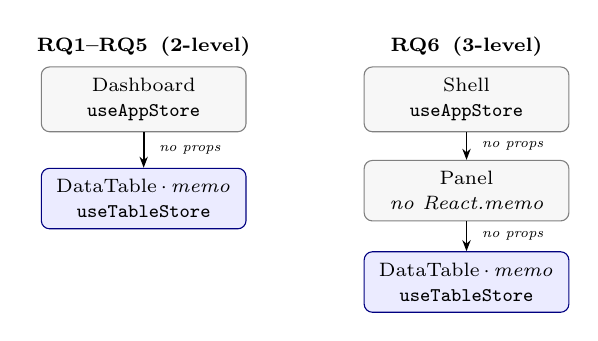
\begin{tikzpicture}[
  box/.style={draw=black!50, rounded corners=3pt, fill=gray!6,
              font=\scriptsize, align=center,
              minimum width=2.6cm, minimum height=0.65cm, inner sep=4pt},
  memo/.style={box, fill=blue!8, draw=blue!50!black},
  arr/.style={-{Stealth[length=4pt,width=3pt]}, semithick},
  lbl/.style={font=\tiny\itshape, right=2pt},
]
  %% 2-level tree (RQ1--RQ5)
  \node[font=\scriptsize\bfseries] at (0, 0.15) {RQ1--RQ5\enspace(2-level)};
  \node[box]  (D)  at (0,-0.52)  {Dashboard\\[1pt]{\ttfamily useAppStore}};
  \node[memo] (DT) at (0,-1.78)
    {DataTable\,$\cdot$\,\textit{memo}\\[1pt]{\ttfamily useTableStore}};
  \draw[arr] (D) -- node[lbl]{no props} (DT);
  %% 3-level tree (RQ6)
  \node[font=\scriptsize\bfseries] at (4.1, 0.15) {RQ6\enspace(3-level)};
  \node[box]  (S)   at (4.1,-0.52)  {Shell\\[1pt]{\ttfamily useAppStore}};
  \node[box]  (P)   at (4.1,-1.68)  {Panel\\[1pt]{\itshape no React.memo}};
  \node[memo] (DT2) at (4.1,-2.84)
    {DataTable\,$\cdot$\,\textit{memo}\\[1pt]{\ttfamily useTableStore}};
  \draw[arr] (S)   -- node[lbl]{no props} (P);
  \draw[arr] (P)   -- node[lbl]{no props} (DT2);
\end{tikzpicture}
\caption{Component tree topologies. Arrows denote parent--child
  relationships; no props cross any edge.
  Blue-shaded nodes carry a \code{React.memo} boundary.}
\label{fig:trees}
\end{figure}

\textbf{Scope note:} The benchmark intentionally uses a minimal
two-component tree to isolate the subscription model as the sole
independent variable; results should be read within this controlled
topology and may not transfer directly to production dashboards with
many independent subscribing components.
\textbf{React Compiler scope boundary:} All measurements use
React~19.1 with the React Compiler~\cite{b13} disabled, which
remains the default configuration as of April~2026. The compiler's
effect on all seven conditions---including proxy incompatibility with
Valtio and MobX---is evaluated in Appendix~\ref{app:compiler}.

The dataset is generated deterministically using a large-prime modulo
(\code{(i * 7919) \% 1000}), with no \code{Math.random()}, so the same
100~rows are produced on every build. The global state shape is defined
by a shared \code{StoreAdapter} interface:

\begin{lstlisting}
export interface StoreAdapter {
  state: AppState    // rows, filter, sortBy, sortDir,
                     // counter, selectedIds
  actions: AppActions
}
\end{lstlisting}

All four library implementations satisfy this interface. The component
tree references only \code{StoreAdapter}, making all JSX byte-for-byte
identical across builds; any observable difference is attributable
solely to the state layer. The 100-row dataset falls below the threshold
at which virtual scrolling is typically introduced, preventing
visualization behaviour from conflating re-render counts. The 100-row
count was selected to represent a realistic dense-table workload;
commonly used virtualisation libraries (e.g., TanStack Virtual, React
Window) are applied at substantially larger row counts, typically
hundreds to thousands of rows. The impact of row count on reconciliation
cost is not independently varied in this study; results should be
interpreted within the non-virtualised dense-render regime.

\subsection{Library Isolation}

Each library is an independent entry point under \code{store/}. The
active entry is selected at build time via a webpack module alias in
\code{next.config.mjs}:

\begin{lstlisting}
config.resolve.alias[
  path.resolve('./store/active.tsx')
] = path.resolve(
  `./store/${process.env.NEXT_PUBLIC_STATE_LIBRARY}/index.tsx`
)
\end{lstlisting}

The alias key is the \textbf{absolute filesystem path} of
\code{store/active.tsx} (see Appendix~\ref{app:webpack} for the
rationale). This enables genuine tree-shaking: only the selected
library's code is included in the output. Each benchmark run begins with
\code{rm -rf .next} to prevent stale chunk reuse.

\subsection{Render Tracking}

\code{Dashboard} and \code{DataTable} are instrumented with a
\code{<RenderTracker id>} wrapper whose \code{useEffect} (no
dependency array) fires after every render commit and pushes a record to
\lstinline|window.__renderRecords|. Playwright reads this array via
\code{page.evaluate()} after each scenario.

React's \code{<Profiler>} API~\cite{b14} was evaluated as an alternative.
In standard \code{react-dom} production builds the \code{onRender}
callback is a no-op; \code{react-dom/profiler} adds instrumentation
overhead that would perturb the measured artifact. The \code{useEffect}
approach avoids this. The trade-off is that render~\emph{duration}
(\code{actualDuration}) is unavailable; render~\emph{count} is
therefore the primary dependent variable. A secondary
\emph{scenario elapsed time} metric (termed render-span for brevity)
approximates per-scenario wall-clock cost as the elapsed time between
the first and last \code{performance.now()} timestamps in
\lstinline|window.__renderRecords| for a given component.
\textbf{Interpretation note:} this metric encompasses React
reconciliation, browser paint, Playwright input dispatch, and
inter-event idle time; it is \emph{not} an isolated measure of
reconciliation CPU cost (React~18 automatic batching~\cite{b5}
requires explicit \code{await} gaps between interactions, and these
idle gaps are included in scenario elapsed time).
Table~\ref{tab:timing} reports mean [95\%~CI] over~$N{=}20$~runs
(run~1 excluded as warm-up; $N{=}19$ steady-state observations;
$t$-distribution, $df{=}18$~\cite{b10}).  The
\code{performance.now()} timestamps are recorded inside
\code{useEffect} callbacks (after each browser paint) and are
React-internal, not Playwright-internal.  In RQ1, Context's 50
\code{useEffect} invocations capture the full wall-clock span
including all inter-click idle time, so render-span measures scenario
elapsed time rather than isolated reconciliation CPU cost.

\subsection{Subscription Scoping Design}
\label{sec:subscriptions}

Global state has two semantically independent regions: \emph{table
state} (\code{rows}, \code{filter}, \code{sortBy}, \code{sortDir},
\code{selectedIds}) and \emph{counter state} (\code{counter}). Each
library exposes two public hooks. \code{useAppStore()} subscribes to
all of \code{AppState} and is used by \code{Dashboard}.
\code{useTableStore()} subscribes to table state only,
excluding~\code{counter}, and is used by \code{DataTable}, which is
also wrapped in \code{React.memo}:

\begin{lstlisting}
export const DataTable = memo(function DataTable() {
  const { rows, filter, sortBy, sortDir,
          selectedIds, toggleSelect } = useTableStore()
  // ...
})
\end{lstlisting}

\textbf{Both conditions are required for render isolation under RQ1.} \code{useTableStore()} prevents the library's
subscription from firing when only~\code{counter} changes.
\code{React.memo} prevents React's reconciliation cascade when
\code{Dashboard} (the parent, subscribed to~\code{counter}) re-renders.
Either condition alone is insufficient.\footnote{Redux's
\code{useAppStore()} uses a single \code{useSelector((s) => s.app)}
call. Because RTK's \code{immer} produces a new object reference on
every dispatch, \code{Dashboard} re-renders on all five scenario types
equally. This asymmetry does not affect \code{DataTable} counts
(Table~\ref{tab:datatable}), which use \code{useTableStore()} with
consistent per-field resolution. The coarser selector is preserved
intentionally as a common pre-optimisation adoption pattern. Note that
this pattern does \emph{not} conform to the Redux Style Guide~\cite{b7},
which recommends per-field selectors; \code{Dashboard}-level
render counts therefore measure Redux under a common footgun rather than
its idiomatic best case. A per-field \code{useAppStore()} variant is
identified as a fifth condition in this study
(\code{redux-idiomatic}; results in Table~\ref{tab:datatable}).}

For Context, \code{useTableStore()} still reads \code{useContext(StateCtx)},
which fires on \emph{any} context value change regardless of which
property changed, the architectural property under test in RQ1. A
dual-context split (\code{StateCtx} and \code{DispatchCtx}) is employed,
a common optimisation that does not change the RQ1 outcome.

\textbf{Zustand~v5 selector pitfall (important for replication):}
Zustand~v5 uses \code{Object.is} for selector equality. Inline
object-literal selectors (e.g., \code{useStore(s => (\{a: s.a\}))}) always
produce new references and cause infinite re-render loops; this is a
silent runtime defect, not a compile-time error. Per-field primitive
selectors are safe; object-returning selectors require \code{useShallow}.
This constraint was applied throughout the benchmark implementation.

\subsection{Interaction Scenarios}
\label{sec:method-timing}

Thirteen research questions (RQ1--RQ13) are covered
(Table~\ref{tab:scenarios}). RQ1--RQ5 operate on the primary two-level
tree; RQ6 uses a dedicated three-level route (\code{Shell} $\to$
\code{Panel} $\to$ \code{DataTable}) with an unmemoised intermediate
component to test whether leaf isolation holds across a deeper tree; RQ7
exercises partial single-field row patches; RQ8 measures K-consumer
fan-out at $K{=}1$, $K{=}3$, and $K{=}10$ (three sub-conditions).  RQ9
extends the depth study with three additional unmemoised intermediate
layers (five-level tree). RQ10 tests Jotai atom-family per-row
isolation outside the uniform \code{StoreAdapter} interface.  Three
further scenarios (RQ11--RQ13) test a \emph{multi-panel topology}:
three independently memoised panels each subscribe to a disjoint state
slice (PanelA~$\to$~counter; PanelB~$\to$~filter/sort/rows;
PanelC~$\to$~selection), exercising whether selector-based libraries
confine re-renders to the panel whose slice actually changed.

\begin{table}[tb]
\caption{Interaction Scenarios and Research Questions}
\label{tab:scenarios}
\begin{center}
\scriptsize
\setlength{\tabcolsep}{4pt}
\begin{tabular}{llrl}
\toprule
\textbf{Scenario} & \textbf{Interaction}         & \textbf{Ops} & \textbf{Metric} \\
\midrule
RQ1 & Counter increment               & 50  & \code{DataTable} re-renders \\
RQ2 & Filter input (keystrokes)        & 5   & \code{DataTable} re-renders \\
RQ3 & Row selection toggle             & 20  & \code{DataTable} re-renders \\
RQ4 & Sort direction toggle            & 10  & \code{DataTable} re-renders \\
RQ5 & Row dataset refresh              & 5   & \code{DataTable} re-renders \\
RQ6 & Counter increment (3-level tree) & 50  & All 3 components \\
RQ7 & Single-field row patch           & 10  & Dashboard + DataTable \\
RQ8 & K-consumer fan-out ($K{=}1,3,10$) & 50  & Total surplus renders \\
RQ9 & Counter incr.\ (5-level deep tree) & 50 & All 5 components \\
RQ10 & Single-field row patch (atom-family) & 10 & Per-row re-renders \\
RQ11 & Counter incr.\ (3-panel multi-slice) & 50 & Per-panel re-renders \\
RQ12 & Filter input (3-panel multi-slice)   & 5  & Per-panel re-renders \\
RQ13 & Row selection (3-panel multi-slice)  & 20 & Per-panel re-renders \\
\bottomrule
\end{tabular}
\end{center}
\end{table}

All interactions are sequentialised with \code{await} to prevent
React~18 automatic batching. In RQ2, \code{pressSequentially('Alpha},
\code{\{delay: 50\})} ensures each keystroke is committed as a separate
React update cycle before the next is dispatched. Assertions are exact
(\code{toBe(n)}): because all interactions are deterministically
scripted, render counts are invariant by construction, and exact
assertions enforce this invariance.

Scenarios execute in fixed order RQ1--RQ7 for the render-count suite
(render counts are deterministic and exact regardless of trial order;
assertions enforce this invariance via \code{toBe(n)}). For the
render-span timing suite, the five RQ1--RQ5 scenario bodies are
executed in a \emph{per-run randomised order} within a single combined
Playwright test using a seeded deterministic shuffle
(linear-congruential PRNG, seed = run index). All five code paths are
thus executed in each of the $N{=}20$ runs before steady-state
observations are drawn, providing a single cross-scenario JIT warm-up
run (run~0) after which V8 has JIT-compiled all paths. Runs 1--19
($N{=}19$ steady-state observations) each present the five scenarios in
a distinct, deterministic order, distributing any residual V8
tier-up or CPU frequency scaling effects across all scenarios rather
than confounding position-dependent scenarios.

\subsection{Bundle Size Measurement}
\label{sec:environment}

Bundle size is measured as First Load JS delta above the 102~KB shared
baseline, as reported by \code{next build}. All primary comparisons use
\textbf{uncompressed} First Load JS; gzip totals of
\code{.next/static/chunks} are a secondary cross-check. Bundle sizes
were verified stable across $N{=}3$ independent clean builds per library
(byte-identical output, consistent with~\cite{b10}). Timing runs use
$N{=}20$ (run~1 excluded as warm-up; $N{=}19$ steady-state observations)
to support formal 95\% confidence interval construction.

The test environment was a MacBook Pro 14-inch (Apple M5~Max, 128~GB
unified memory) running macOS~26.4~Tahoe, Node.js~v22.14.0, and
pnpm~v9.15.4. Primary benchmark runs used Playwright~1.59.1 with
Chromium (V8); the Firefox cross-validation run used
Firefox~148.0.2 (SpiderMonkey) via Playwright's \textit{Desktop Firefox}
device profile (Appendix~\ref{app:firefox}). \textbf{Hardware note:
Absolute render-span values scale with hardware speed.}  The Apple
M5~Max represents an unusually high-performance configuration;
absolute values in Table~\ref{tab:timing} are expected to be
substantially longer on mid-range x86-class hardware (developer
laptops, CI runners, cloud VMs).  Absolute render-span results should
therefore be treated as lower bounds on timing for comparable
hardware; relative comparisons \emph{within a single hardware
platform} are unaffected by machine speed.  The render-\emph{count}
results (Tables~\ref{tab:datatable}--\ref{tab:rq6}) are
hardware-independent.
Cross-hardware replication on three additional platforms (an
Apple~M3~Max 128~GB MacBook Pro, independent collaborator machine; an
Intel~Core~i9 MacBook Pro; and an Apple~M1 GitHub Actions runner) is
reported in Appendix~\ref{app:crosshw}.

% ── IV. Results ───────────────────────────────────────────────────────────────
\section{Results}
\label{sec:results}

\subsection{Bundle Overhead}

Table~\ref{tab:bundle} reports uncompressed First Load JS and the delta
above the 102~KB shared baseline. All three independent clean builds per
library produced byte-identical figures, confirming webpack output
determinism. Fig.~\ref{fig:bundle} visualises the deltas.

\begin{table}[tb]
\caption{Bundle Overhead Per Library. Primary: First Load JS delta
above 102~KB shared baseline. React Context has \textbf{zero} external
library overhead; its 104~KB total is indistinguishable from the baseline
at 1-KB reporting precision; the nominal +2~KB reflects benchmark
adapter code present in all configurations, not an npm
dependency.$^{\dagger}$}
\label{tab:bundle}
\begin{center}
\small
\setlength{\tabcolsep}{4pt}
\begin{tabular}{lccc}
\toprule
\textbf{Library}               & \textbf{First Load} & \textbf{Delta} & \textbf{Gzip} \\
\midrule
Redux Toolkit v2.5 (coarse)    & 112~KB & \textbf{+10~KB} & 244.5~KB \\
Redux Toolkit v2.5 (idiomatic) & 112~KB & \textbf{+10~KB} & 244.7~KB \\
Jotai v2.12                    & 107~KB & \textbf{+5~KB}  & 240.0~KB \\
Zustand v5.0                   & 104~KB & \textbf{+2~KB}  & 238.0~KB \\
React Context (built-in)       & 104~KB & \textbf{0~KB}$^{\dagger}$ & 237.2~KB \\
Valtio v2.3 (proxy)            & 105~KB & \textbf{+3~KB}  & 245.9~KB \\
MobX v6.15 (observable)        & 119~KB & \textbf{+17~KB} & 260.1~KB \\
\bottomrule
\end{tabular}
\end{center}
\parbox{\columnwidth}{\scriptsize $^{\dagger}$Context is a built-in React
primitive with no npm dependency. The 2~KB above the 102~KB baseline is
benchmark adapter code common to all configurations.}
\end{table}

\begin{figure}[tb]
  \centering
  \includegraphics[width=\columnwidth]{figure2.pdf}
  \caption{Bundle overhead delta per library (uncompressed First Load
  JS). Lower is better. Context's bar reflects benchmark adapter code
  common to all configurations; the library itself adds 0~KB (see
  Table~\ref{tab:bundle}).}
  \label{fig:bundle}
\end{figure}

Redux's +10~KB overhead reflects RTK's action-creator utilities,
reducer helpers, and \code{immer}. Although RTK bundles
\code{reselect}, the benchmark does not call \code{createSelector}, so
\code{reselect} contributes zero to the delta. Redux's per-route chunk
(2.10~KB) is \emph{smaller} than Zustand's (2.49~KB), yet its First
Load JS total is 8~KB larger: RTK's dependencies land in shared chunks
loaded on every navigation, inflating First Load JS without appearing in
the per-route chunk. This illustrates that per-route chunk size is a
misleading bundle metric when dependency graphs are hoisted into shared
chunks; First Load JS, which subsumes all shared-chunk contributions,
is the more accurate measure of delivery cost. A symmetric
shared-chunk breakdown for Jotai and Zustand was not conducted; the
reported First Load JS figures capture each library's full contribution
but do not separate per-route from shared-chunk portions. The two Redux variants share a nearly byte-identical bundle (+10~KB each);
the second variant adds only per-field
\code{useSelector} calls and contributes no additional dependency weight.
\textbf{Context bundle cost.} React Context is a built-in React
primitive carrying zero external library overhead. Its 104~KB First
Load JS equals the Zustand total in absolute terms; however, Zustand's
+2~KB delta represents a genuine npm dependency whereas Context's same
nominal delta is entirely benchmark adapter code common to all
configurations. In bundle terms, Context is effectively free.
Gzip totals (Table~\ref{tab:bundle}) broadly track uncompressed deltas:
MobX ($260.1$~KB) $>$ Valtio ($245.9$~KB) $>$ Redux ($244.5$~KB) $>$
Jotai ($240.0$~KB) $>$ Zustand ($238.0$~KB) $\approx$ Context ($237.2$~KB),
confirming consistency across measurement methods.
Note that Valtio's gzip rank (above Redux) exceeds its uncompressed-delta
rank ($+3$~KB vs.~$+10$~KB): proxy-polyfill code compresses less
efficiently than Redux Toolkit's action-creator utilities.
\textbf{Valtio and MobX bundle cost.} Valtio~(v2.3) adds $+3$~KB above
the 102~KB shared baseline, ranking between Zustand ($+2$~KB) and
Jotai ($+5$~KB) by uncompressed delta. MobX~(v6.15) adds $+17$~KB---the
largest overhead of the tested libraries---reflecting \code{mobx}'s
reactive data engine and \code{mobx-react-lite}'s observer context.

\subsection{Re-render Counts}

Table~\ref{tab:datatable} reports \code{DataTable} re-render counts per
scenario and library. Table~\ref{tab:dashboard} reports \code{Dashboard}
counts (identical across all seven tested conditions), validating
measurement calibration. \textbf{Design note:} Redux's \code{useAppStore()} uses a
deliberately coarse selector, \code{(s) => s.app}, rather than
per-field selectors. This is a common initial adoption pattern before
per-field memoisation is introduced, but it does \emph{not} conform to
the Redux Style Guide~\cite{b7}, which recommends per-field selectors.
\textbf{\code{Dashboard}-level render counts (Table~\ref{tab:dashboard})
therefore measure Redux under a common pre-optimisation pattern
(\emph{not} its idiomatic best case) and should not be used in
isolation to assess Redux's render-count performance.}
\code{DataTable} counts (Table~\ref{tab:datatable}) are unaffected:
\code{useTableStore()} applies consistent per-field resolution across
all libraries.\footnote{In the tested scenarios all dispatches
modify at least one field of \code{s.app}, so the coarse selector
produces identical \code{Dashboard} counts to per-field subscriptions.
A per-field Redux \code{useAppStore()} variant is included as a fifth
condition in this study (\code{redux-idiomatic}; results in
Table~\ref{tab:datatable}).}
Table~\ref{tab:timing} reports inter-library render-span timing.

\begin{table}[tb]
\caption{\code{DataTable} Re-render Counts Per Scenario and Library.
  Valtio~(v2.3) and MobX~(v6.15) replications confirmed identical;
  see Table~\ref{tab:replications}.}
\label{tab:datatable}
\begin{center}
\small
\setlength{\tabcolsep}{4pt}
\begin{tabular}{lccccc}
\toprule
\textbf{Scenario}             & \textbf{Redux} & \textbf{Rdx-Idm}
                              & \textbf{Jotai} & \textbf{Zustand} & \textbf{Context} \\
\midrule
RQ1 --- counter $\times$50   & \textbf{0}  & \textbf{0}  & \textbf{0}  & \textbf{0}  & \textbf{50} \\
RQ2 --- filter $\times$5     & 5  & 5  & 5  & 5  & 5  \\
RQ3 --- select $\times$20    & 20 & 20 & 20 & 20 & 20 \\
RQ4 --- sort $\times$10      & 10 & 10 & 10 & 10 & 10 \\
RQ5 --- rows $\times$5       & 5  & 5  & 5  & 5  & 5  \\
RQ7 --- patch $\times$10     & 10 & 10 & 10 & 10 & 10 \\
\bottomrule
\end{tabular}
\end{center}
\end{table}

\begin{table}[tb]
\caption{\code{Dashboard} Re-render Counts Per Scenario and Library
(identical across all libraries, validates measurement calibration)}
\label{tab:dashboard}
\begin{center}
\small
\setlength{\tabcolsep}{4pt}
\begin{tabular}{lccccc}
\toprule
\textbf{Scenario}             & \textbf{Redux} & \textbf{Rdx-Idm}
                              & \textbf{Jotai} & \textbf{Zustand} & \textbf{Context} \\
\midrule
RQ1 --- counter $\times$50   & 50 & 50 & 50 & 50 & 50 \\
RQ2 --- filter $\times$5     & 5  & 5  & 5  & 5  & 5  \\
RQ3 --- select $\times$20    & 20 & 20 & 20 & 20 & 20 \\
RQ4 --- sort $\times$10      & 10 & 10 & 10 & 10 & 10 \\
RQ5 --- rows $\times$5       & 5  & 5  & 5  & 5  & 5  \\
RQ7 --- patch $\times$10     & 10 & 10 & 10 & 10 & 10 \\
\bottomrule
\end{tabular}
\end{center}
\end{table}

\begin{table}[tb]
\caption{Valtio (v2.3) and MobX (v6.15) Render-Count Replication
  (primary route, M5~Max). Both proxy/observable libraries produce
  counts byte-identical to the selector-based primary conditions
  (Table~\ref{tab:datatable}). RQ6 (depth~3), RQ9 (depth~5), and
  RQ8 fan-out confirmed: Shell/Panel/layers~$=$~50, DataTable~$=$~0,
  surplus~$=$~0 at $K{=}3$ and $K{=}10$. Tests: 12/12 each.
  Timing ($N{=}20$, same steady-state protocol) reported in Table~\ref{tab:timing}.}
\label{tab:replications}
\begin{center}
\small
\setlength{\tabcolsep}{4pt}
\begin{tabular}{lcccc}
\toprule
\textbf{Scenario}
  & \multicolumn{2}{c}{\textbf{Dashboard}}
  & \multicolumn{2}{c}{\textbf{DataTable}} \\
\cmidrule(lr){2-3}\cmidrule(lr){4-5}
  & \textbf{Valtio} & \textbf{MobX}
  & \textbf{Valtio} & \textbf{MobX} \\
\midrule
RQ1 --- counter $\times$50   & 50 & 50 & \textbf{0} & \textbf{0} \\
RQ2 --- filter $\times$5     & 5  & 5  & 5  & 5  \\
RQ3 --- select $\times$20    & 20 & 20 & 20 & 20 \\
RQ4 --- sort $\times$10      & 10 & 10 & 10 & 10 \\
RQ5 --- rows $\times$5       & 5  & 5  & 5  & 5  \\
RQ7 --- patch $\times$10     & 10 & 10 & 10 & 10 \\
\bottomrule
\end{tabular}
\end{center}
\end{table}

\begin{table*}[tb]
\caption{Supplementary: \code{DataTable} Scenario Elapsed Time
  (Indicative Wall-Clock Cost).
  Mean [$\pm$95\%~CI] in~ms, $N{=}19$ steady-state runs
  ($t$-distribution, $df{=}18$, run~1 excluded as warm-up~\cite{b10}).
  Render count (Table~\ref{tab:datatable}) is the primary dependent
  variable; this table approximates scenario-level wall-clock cost and
  encompasses Playwright overhead, event propagation, and inter-event
  idle time --- it is not an isolated reconciliation measure.
  \texttt{---} indicates zero renders (RQ1 selector-based libraries).
  The RQ1 Context value (1632.1~ms) is hardware-dependent; see
  Table~\ref{tab:timing-hw} for cross-platform comparisons.
  Scenario order is randomised per run (seeded deterministic shuffle,
  seed = run index); inter-library comparisons within each scenario
  row are valid; cross-scenario comparisons are indicative only
  (see Sections~\ref{sec:methodology} and~\ref{sec:threats}).
  For RQ2--RQ5, sub-2~ms inter-library deltas primarily confirm
  test harness consistency across library runs rather than isolating
  reconciliation CPU cost.
  \textbf{Rdx-Idm} = \code{redux-idiomatic} (per-field
  \code{useSelector} at \code{Dashboard} level; see
  Section~\ref{sec:threats}).
  Valtio and MobX timing collected in a dedicated $N{=}20$ pass
  (same steady-state protocol; run~1 warm-up excluded).}
\label{tab:timing}
\begin{center}
\small
\setlength{\tabcolsep}{3pt}
\begin{tabular}{lccccccc}
\toprule
\textbf{Scenario}
  & \textbf{Redux}
  & \textbf{Rdx-Idm}
  & \textbf{Jotai}
  & \textbf{Zustand}
  & \textbf{Context}
  & \textbf{Valtio}
  & \textbf{MobX} \\
\midrule
RQ1 --- counter $\times$50
  & ---
  & ---
  & ---
  & ---
  & $1632.1\,[\pm 0.5]$
  & ---
  & --- \\
RQ2 --- filter $\times$5
  & $213.2\,[\pm 0.7]$
  & $212.9\,[\pm 1.5]$
  & $213.7\,[\pm 0.7]$
  & $212.6\,[\pm 1.2]$
  & $213.0\,[\pm 0.7]$
  & $211.7\,[\pm 0.9]$
  & $212.3\,[\pm 0.9]$ \\
RQ3 --- select $\times$20
  & $632.0\,[\pm 0.6]$
  & $631.4\,[\pm 0.7]$
  & $631.5\,[\pm 0.6]$
  & $631.7\,[\pm 0.6]$
  & $631.9\,[\pm 0.7]$
  & $632.9\,[\pm 1.9]$
  & $631.4\,[\pm 1.0]$ \\
RQ4 --- sort $\times$10
  & $297.5\,[\pm 0.6]$
  & $297.2\,[\pm 0.6]$
  & $297.5\,[\pm 0.4]$
  & $298.3\,[\pm 2.1]$
  & $298.1\,[\pm 1.8]$
  & $297.9\,[\pm 0.6]$
  & $297.5\,[\pm 1.9]$ \\
RQ5 --- rows $\times$5
  & $131.7\,[\pm 0.5]$
  & $131.9\,[\pm 0.6]$
  & $131.7\,[\pm 0.7]$
  & $131.7\,[\pm 0.5]$
  & $131.1\,[\pm 0.5]$
  & $130.8\,[\pm 0.5]$
  & $130.5\,[\pm 0.4]$ \\
\bottomrule
\end{tabular}
\end{center}
\end{table*}

\textbf{RQ1} yields the study's primary finding: Context produced 50
surplus re-renders; all six selector-based conditions (Redux,
redux-idiomatic, Jotai, Zustand, Valtio, and MobX) produced
zero: a complete elimination of wasted work. Each counter increment
changes \code{StateCtx}'s value object, propagating to all
\code{useContext(StateCtx)} consumers regardless of which properties
changed. Redux, Zustand, Jotai, Valtio, and MobX each detect that
their subscribed
fields (\code{rows}, \code{filter}, \code{sortBy}, \code{sortDir},
\code{selectedIds}) have not changed and skip the render entirely (see
Section~\ref{sec:subscriptions}). The 1632~ms render-span for Context
represents the wall-clock time across the full 50-increment sequence
(including inter-click idle time) during which \code{DataTable}'s
reconciliation is invoked on all 50 passes that the selector-based
libraries avoid.  This 1632~ms figure is a scenario-level wall-clock
total encompassing Playwright input dispatch, event propagation, commit
scheduling, and inter-click idle; it should \emph{not} be read as pure
reconciliation overhead (see Section~\ref{sec:discussion} for
contextual scale framing).
Because render counts are enforced as exact deterministic assertions
(\code{toBe($n$)} in Playwright), they carry no sampling uncertainty
and require no statistical interval: the count either passes or the
test suite fails.

\textbf{RQ2--RQ5} produce identical counts across all seven tested
conditions (5, 20, 10, and~5 respectively). When the changed state
\emph{is} consumed by the subscribing component, there is no wasted
rendering regardless of library. The performance advantage of
selector-based subscription is strictly zero in these scenarios.

\textbf{RQ6} tests render isolation in a three-level tree where the
intermediate component (\code{Panel}) is deliberately \emph{not} wrapped
in \code{React.memo} (Table~\ref{tab:rq6}). \code{Shell} re-renders once
per counter increment for all six selector-based conditions;
\code{Panel} cascades 50 re-renders from the parent, also uniformly.
\code{DataTable}'s \code{React.memo} bail-out fires for all
selector-based conditions (zero renders), while Context produces~50.
This confirms that render isolation at a memoised leaf survives
intermediate unmemoised layers.

\begin{table}[tb]
\caption{RQ6 --- Re-render Counts Across All Three Levels of the Nested
Tree (50 Counter Increments).}
\label{tab:rq6}
\begin{center}
\scriptsize
\setlength{\tabcolsep}{2pt}
\begin{tabular}{lccccccc}
\toprule
\textbf{Component} & \textbf{Rdx} & \textbf{RI} & \textbf{Jtai}
  & \textbf{Zstd} & \textbf{Valt} & \textbf{MobX} & \textbf{Ctx} \\
\midrule
Shell (root)     & 50 & 50 & 50 & 50 & 50 & 50 & 50 \\
Panel (no memo)  & 50 & 50 & 50 & 50 & 50 & 50 & 50 \\
DataTable (leaf) & \textbf{0} & \textbf{0} & \textbf{0} & \textbf{0}
                 & \textbf{0} & \textbf{0} & \textbf{50} \\
\bottomrule
\end{tabular}
\end{center}
\parbox{\columnwidth}{\scriptsize
  Rdx=Redux, RI=\code{redux-idiomatic}, Jtai=Jotai, Zstd=Zustand,
  Valt=Valtio, Ctx=Context.}
\end{table}

\textbf{RQ9} extends the depth study of RQ6 by inserting three
additional unmemoised intermediate layers (\code{Layer1}--\code{Layer3})
between the state-subscribing root (\code{DeepShell}) and the
\code{React.memo}-guarded leaf (\code{DataTable}), producing a
five-level tree.  The five-level route replaces all
five selector-based libraries' \code{DataTable} re-renders with 0, while Context
continues to produce 50 (Table~\ref{tab:deep}).  The result
extends the RQ6 depth-invariance finding: \code{React.memo} isolation
at a leaf survives arbitrary numbers of unmemoised intermediate layers,
regardless of tree depth.

\begin{table}[tb]
\caption{RQ9 --- Re-render Counts in the 5-Level Tree (50 Counter Increments).
  $\mathbf{0}$ entries confirm \code{React.memo} leaf isolation persists
  through three additional unmemoised intermediate layers.}
\label{tab:deep}
\begin{center}
\scriptsize
\setlength{\tabcolsep}{2pt}
\begin{tabular}{lccccccc}
\toprule
\textbf{Component} & \textbf{Rdx} & \textbf{RI} & \textbf{Jtai}
  & \textbf{Zstd} & \textbf{Valt} & \textbf{MobX} & \textbf{Ctx} \\
\midrule
DeepShell (root)  & 50 & 50 & 50 & 50 & 50 & 50 & 50 \\
Layer1 (no memo)  & 50 & 50 & 50 & 50 & 50 & 50 & 50 \\
Layer2 (no memo)  & 50 & 50 & 50 & 50 & 50 & 50 & 50 \\
Layer3 (no memo)  & 50 & 50 & 50 & 50 & 50 & 50 & 50 \\
DataTable (leaf)  & \textbf{0} & \textbf{0} & \textbf{0} & \textbf{0}
                  & \textbf{0} & \textbf{0} & \textbf{50} \\
\bottomrule
\end{tabular}
\end{center}
\parbox{\columnwidth}{\scriptsize
  Rdx=Redux, RI=\code{redux-idiomatic}, Jtai=Jotai, Zstd=Zustand,
  Valt=Valtio, Ctx=Context.}
\end{table}

\textbf{RQ7}: ten consecutive single-field row patches
(\code{patchRow('row-0', \{value: prev + 1\})}) produced 10
\code{Dashboard} re-renders and 10 \code{DataTable} re-renders across
all seven tested conditions. Although Redux's \code{immer} preserves
unchanged row object references (structural sharing), all seven
\code{useTableStore()} implementations subscribe to the \code{rows}
\emph{array} reference.
Every \code{patchRow()} call produces a new array reference via
\code{.map()}, triggering a re-render in all libraries. The RQ7
equivalence therefore characterises
\emph{all seven conditions subject to
the array-reference subscription constraint of the uniform
\code{StoreAdapter} interface}, not the libraries' intrinsic
capabilities under per-row update workloads.

\textbf{RQ10} tests the per-row subscription capability that lies
\emph{outside} the uniform \code{StoreAdapter} interface.  A dedicated
\code{/atom-family} route implements one Jotai atom per row:
\code{rowAtomMap} stores 100 individual \code{atom<Row>} instances;
each \code{RowCell} component subscribes exclusively to its own row
atom.  Applying 10 consecutive patches to \code{row-0} produced
10~re-renders in \code{RowCell-row-0} and exactly 0~re-renders in
every other \code{RowCell} (rows 1--99) as well as in the
\code{AtomFamilyTable} wrapper (which reads only the stable
\code{rowIdsAtom}).  Compared with RQ7's baseline of 10~\code{DataTable}
re-renders encompassing all 100 rows, the atom-family pattern
triggers reconciliation of only 1 of 100~\code{RowCell} components
per patch; the other 99 remain idle, as does the
\code{AtomFamilyTable} wrapper, confirming the theoretical per-row isolation
advantage of Jotai's atomic subscription model under single-row
update workloads.

\subsection{Multi-Panel Topology (RQ11--RQ13)}

RQ11--RQ13 evaluate whether subscription-level isolation generalises
beyond the canonical two-component Dashboard+DataTable tree to a
\emph{multi-panel topology} in which three independently memoised panels
each subscribe to a disjoint state slice:
\textbf{PanelA}~$\to$~\code{useCounterSlice()} (counter only),
\textbf{PanelB}~$\to$~\code{useFilterSortSlice()} (rows, filter, sortBy, sortDir),
\textbf{PanelC}~$\to$~\code{useSelectionSlice()} (selectedIds).
Each panel is instrumented with a \code{RenderTracker} recording every
render commit; controls outside the panels drive the store
without being tracked.

Table~\ref{tab:multipanel} shows the render counts across all seven
conditions. The result is unambiguous: all six selector-based libraries
(Redux, redux-idiomatic, Zustand, Jotai, Valtio, MobX) produce
\emph{zero} re-renders in the two panels whose slices were not changed,
regardless of which scenario drove the mutation. React Context, with its
all-or-nothing subscription to the shared \code{StateCtx} value, broadcasts
to all three panels on every mutation, producing a $3{\times}$ surplus
in all cross-slice scenarios.

\begin{table}[tb]
\caption{RQ11--RQ13 --- Multi-Panel Render Counts. PA\,=\,PanelA
  (\code{useCounterSlice}), PB\,=\,PanelB (\code{useFilterSortSlice}),
  PC\,=\,PanelC (\code{useSelectionSlice}).
  \textbf{Bold} entries highlight surplus re-renders.}
\label{tab:multipanel}
\begin{center}
\scriptsize
\setlength{\tabcolsep}{3pt}
\begin{tabular}{l|rrr|rrr|rrr}
\toprule
& \multicolumn{3}{c|}{\textbf{RQ11} (50 counter incr.)}
& \multicolumn{3}{c|}{\textbf{RQ12} (5 filter keys)}
& \multicolumn{3}{c}{\textbf{RQ13} (20 sel.\ toggles)} \\
\textbf{Library} & PA & PB & PC & PA & PB & PC & PA & PB & PC \\
\midrule
Redux       & 50 & 0 & 0 & 0 & 5  & 0 & 0 & 0  & 20 \\
Rdx-Idm.    & 50 & 0 & 0 & 0 & 5  & 0 & 0 & 0  & 20 \\
Zustand     & 50 & 0 & 0 & 0 & 5  & 0 & 0 & 0  & 20 \\
Jotai       & 50 & 0 & 0 & 0 & 5  & 0 & 0 & 0  & 20 \\
Valtio      & 50 & 0 & 0 & 0 & 5  & 0 & 0 & 0  & 20 \\
MobX        & 50 & 0 & 0 & 0 & 5  & 0 & 0 & 0  & 20 \\
\midrule
Context     & 50 & \textbf{50} & \textbf{50}
            & \textbf{5} & 5 & \textbf{5}
            & \textbf{20} & \textbf{20} & 20 \\
\bottomrule
\end{tabular}
\end{center}
\parbox{\columnwidth}{\scriptsize Rdx-Idm.\,=\,\code{redux-idiomatic}.
  Bold: surplus renders in panels whose subscribed slice did not change.}
\end{table}

The six selector-based libraries achieve zero surplus renders through
mechanistically different routes: Redux and redux-idiomatic via per-field
\code{useSelector}; Zustand and Jotai via fine-grained per-field or per-atom
selectors; Valtio via per-instance \code{prevValue} closures gating
\code{useSyncExternalStore} notifications; MobX via \code{reaction()} trackers
that observe only the declared slice fields.
The consistent outcome confirms that the multi-panel isolation property is
a consequence of the \emph{field-level subscription contract}, not any
specific library implementation.

% ── V. Discussion ─────────────────────────────────────────────────────────────
\section{Discussion}
\label{sec:discussion}

\subsection{The Render Isolation Tradeoff}

The RQ1 result demonstrates that React Context imposes a render cost
proportional to the state update frequency of \emph{any} slice in the
shared context, not only the slices a component cares about. The RQ6
results confirm that this isolation extends across a three-level tree:
\code{React.memo} at the leaf is sufficient regardless of intermediate
tree depth.

One important nuance: \code{DataTable}'s \code{useMemo} guard
on \code{visibleRows} prevents the filter-and-sort computation from
rerunning during Context's 50 surplus renders, because the Context
reducer preserves stable field references when only \code{counter}
changes. The 50 extra reconciliations incur only React reconciliation
overhead, not recomputation cost. In real applications where a hot state
slice also writes fields consumed by the table (e.g., a WebSocket price
feed updating both a counter and row values simultaneously), the
\code{useMemo} guard would not help and the full O($n \log n$)
recomputation would be incurred on every surplus render.

\textbf{Consumer-count fan-out (RQ8).}
The main benchmark uses a single \code{DataTable} consumer ($K{=}1$).
To empirically validate the $K{\times}N$ scaling claim, I added RQ8:
a dedicated \code{/k-consumer} route renders $K$ identical
\code{React.memo}-wrapped \code{DataTable} instances, each subscribing
to the same store. Table~\ref{tab:kconsumer} reports total surplus
render counts for $K{=}1$, $K{=}3$, and $K{=}10$ under 50 counter
increments. Context's surplus renders scale exactly as $K{\times}N$:
50 at $K{=}1$, 150 at $K{=}3$, and 500 at $K{=}10$. All three
selector-based libraries produce zero surplus renders at every $K$
value tested. Fan-out linear scaling is empirically confirmed: the
cost is proportional to the number of consumers, not to the store
library's subscription overhead.

\begin{table}[tb]
\caption{RQ8 --- K-Consumer Fan-out: Total Surplus Re-render Counts
  Under 50 Counter Increments. Context scales as $K{\times}50$;
  all six selector-based conditions produce zero at every $K$.}
\label{tab:kconsumer}
\begin{center}
\scriptsize
\setlength{\tabcolsep}{2pt}
\begin{tabular}{lccccccc}
\toprule
\textbf{$K$} & \textbf{Rdx} & \textbf{RI} & \textbf{Jtai}
  & \textbf{Zstd} & \textbf{Valt} & \textbf{MobX} & \textbf{Ctx} \\
\midrule
$K{=}1$ (baseline)  & 0 & 0 & 0 & 0 & 0 & 0 & \textbf{50}  \\
$K{=}3$             & 0 & 0 & 0 & 0 & 0 & 0 & \textbf{150} \\
$K{=}10$            & 0 & 0 & 0 & 0 & 0 & 0 & \textbf{500} \\
\bottomrule
\end{tabular}
\end{center}
\parbox{\columnwidth}{\scriptsize
  Rdx=Redux, RI=\code{redux-idiomatic}, Jtai=Jotai, Zstd=Zustand,
  Valt=Valtio, Ctx=Context.}
\end{table}

Redux, Zustand, Jotai, Valtio, and MobX achieve equivalent render
isolation through different mechanisms. The mechanism differs; the
outcome (zero unnecessary re-renders when unrelated state changes) is
identical when each library is used idiomatically. Render-span timing was not collected
for RQ8, as the deterministic count result fully characterises the
fan-out behaviour; wall-clock cost scales linearly from the per-render
latency reported in Table~\ref{tab:timing}. One practical point worth emphasising:
\code{React.memo} is a \emph{necessary partner} to field-level subscriptions
when the parent subscribes to the changing state slice.
Without it, parent re-renders cascade to all children regardless of
subscription scope.
Alternative topology patterns that place consumers \emph{outside} the
re-rendering subtree (i.e., no ancestor of the consumer subscribes to
the changing slice) can achieve isolation without memoisation; this
benchmark uses the parent-child topology because it represents the most
common production dashboard pattern.

\subsection{Bundle Size vs.\ Runtime Render Cost}

For applications where state slices update together or infrequently
(CRUD, form-heavy, content management), Context's RQ1 overhead is
rarely observable, and its zero-overhead bundle profile makes it a
strong default choice.

For applications with high-frequency independent state updates (real-time
dashboards, multiplayer tools, data feeds), Redux, Zustand, or Jotai
provide meaningful runtime savings at the cost of a small bundle
increase. Among the three, Zustand's +2~KB overhead makes it the most
cost-efficient choice when atomic state (Jotai) or Redux's ecosystem
(DevTools, middleware, code generation) is not required.

The avoidable scenario-level overhead incurred by Context in RQ1 is
$1632.1$~ms (M5~Max, Table~\ref{tab:timing}) versus $0.0$~ms for all
four selector-based libraries over the same 50-increment burst;
the M3~Max figure is $1634.2$~ms (Table~\ref{tab:timing-hw}).
\textbf{Interpretation caveat:} these totals encompass Playwright input
dispatch, event propagation, commit scheduling, and inter-click idle
time.  Dividing the scenario total by the render count to derive a
per-render reconciliation cost is not meaningful: the denominator
(50~React commits) does not correspond to the numerator (scenario
elapsed time including idle), so the quotient does not isolate
reconciliation CPU cost.  At $1.6$~seconds of scenario-level overhead
for a 50-increment burst (consistent across M5~Max and M3~Max), the
surplus is macroscopically user-visible under high-frequency update
workloads.

Tables~\ref{tab:framework} and~\ref{tab:practitioner} translate these
findings into a practical decision framework. Table~\ref{tab:framework} contains only
rows whose Evidence column cites a specific measurement from this paper;
Table~\ref{tab:practitioner} contains guidance rooted in community
convention and library documentation.

\begin{table*}[tb]
\caption{Empirically Supported Decision Framework (all rows are
directly measured in this study)}
\label{tab:framework}
\begin{center}
\small
\setlength{\tabcolsep}{5pt}
\begin{tabular}{p{4.2cm}p{2.8cm}p{2.8cm}p{4.2cm}}
\toprule
\textbf{Usage profile} & \textbf{Recommended} & \textbf{Evidence} & \textbf{Note} \\
\midrule
High-frequency updates to independent slices (dashboards, real-time feeds)
  & Redux / Zustand / Jotai
  & RQ1: 0 vs.\ 50 re-renders
  & Zustand (+2~KB) delivers identical isolation at 20\% of Redux's bundle cost (+10~KB) \\
Bundle-constrained; infrequent cross-slice updates
  & React Context
  & RQ1--RQ5, Table~\ref{tab:bundle}
  & \\
Smallest external library overhead
  & Zustand
  & Table~\ref{tab:bundle}: +2~KB
  & \\
Row dataset replacement (full array refresh)
  & All libraries equivalent
  & RQ5: 5 renders each
  & Subscribed to \code{rows} array reference; new reference on every refresh \\
Single-field partial row patch (array-reference subscription)
  & All libraries equivalent under \code{StoreAdapter}
  & RQ7: 10 full-table re-renders each
  & Uniform \code{StoreAdapter} interface subscribes to the \code{rows}
    array reference; every \code{patchRow()} replaces the array,
    triggering a full \code{DataTable} re-render in all libraries \\
High-frequency per-row updates; independent row subscriptions
  & Jotai atom families
  & RQ10: only the affected \code{RowCell} re-renders; all 99 unaffected
    \code{RowCells} and \code{DataTable} remain idle
  & One \code{atom<Row>} per row; each \code{RowCell} subscribes to its
    own atom; wrapper component reads only stable \code{rowIdsAtom} \\
\bottomrule
\end{tabular}
\end{center}
\end{table*}

\begin{table}[tb]
\caption{Practitioner Guidance (Not Directly Measured in This Study)}
\label{tab:practitioner}
\begin{center}
\small
\setlength{\tabcolsep}{4pt}
\begin{tabular}{p{2.4cm}p{2.4cm}p{2.0cm}}
\toprule
\textbf{Consideration} & \textbf{Guidance} & \textbf{Basis} \\
\midrule
Large team; DevTools workflow & Redux Toolkit & Convention~\cite{b7} \\
Minimal API surface            & Zustand        & Docs~\cite{b2} \\
Complex derived/atomic state   & Jotai          & Docs~\cite{b3} \\
\bottomrule
\end{tabular}
\end{center}
\end{table}

\subsection{React Compiler Compatibility}
\label{sec:compiler}

An unexpected secondary finding emerges from enabling the React
Compiler~\cite{b13} (\code{babel-plugin-react-compiler}~v1.0.0) across
all seven conditions.  Proxy-based libraries (Valtio, MobX) are
\emph{incompatible} with the current compiler: its static
dependency-graph analysis cannot resolve which fields a component
accesses through a runtime proxy, producing over-aggressive memoisation
that \emph{suppresses required re-renders}.  Under Valtio,
\code{DataTable} renders are incorrectly skipped in RQ3 (selection:
$20{\to}0$); under MobX, \emph{all} component renders collapse to~0
across every scenario.  Both failures are silent---no compilation error
or runtime warning is emitted---making the incompatibility invisible to
standard production monitoring.
Practitioners adopting proxy-based reactive libraries should disable
the React Compiler for store-consuming components until explicit
framework support is provided.

For the five compiler-compatible conditions (Redux, redux-idiomatic,
Zustand, Jotai, Context), the compiler \emph{fully eliminates} all
surplus re-renders without code changes: Context~RQ1 timing drops from
$1\,632$~ms to $0.0$~ms; intermediate unmemoised layers (Panel in RQ6,
Layer1--3 in RQ9) are auto-memoised across all four selector-based
conditions.  When the compiler is enabled, the runtime distinction
between Context and selector-based libraries is erased for
compiler-compatible workloads.  Full data are in
Appendix~\ref{app:compiler}.

\subsection{Threats to Validity}
\label{sec:threats}

\textbf{Internal validity.} Each scenario exercises a single interaction
type in isolation. The 100-row dataset does not generalise uniformly
to all table sizes.
\textbf{Render count} is determined solely by the library's
subscription model and is invariant to row count: selector-based
libraries produce 0 surplus renders on a counter increment regardless
of whether 100 or 10\,000 rows sit in the store.
What scales with row count is the per-render reconciliation
\emph{cost}: as the DOM-visible row count grows toward the
virtual-scrolling activation threshold, each surplus render becomes
proportionally more expensive.
At row counts where virtual scrolling activates (typically
$>$200--300 visible rows), the rendered-row count is capped by viewport
capacity rather than store size, bounding each pass.
The RQ1 finding (zero vs.\ 50 surplus re-renders) is therefore
invariant to row count; absolute timing of the
surplus is not. RQ7
exercises single-field patches at the array-reference level; Jotai
row-level atom subscriptions are excluded by the uniform
\code{StoreAdapter} interface. Render-count scenarios execute in fixed
order (RQ1--RQ7); timing scenarios use a per-run randomised order
(seeded deterministic shuffle, Section~\ref{sec:method-timing}), so
residual ordering effects on CPU frequency scaling and JIT warm-up state
are distributed across libraries and captured within the reported
confidence intervals. The deterministic dataset's regular structure (five evenly
distributed categories, prime-modulo value distribution) produces fixed
filter-selectivity ratios under RQ2; variable selectivity (matching 2
vs.\ 98 of 100 rows) may produce different reconciliation profiles
through the \code{useMemo}-guarded filter step, an interaction not
explored in this study.

\textbf{External validity.} The benchmark uses Next.js~15 with
statically pre-rendered pages and does not cover dynamic SSR, React
Server Components, or Concurrent Mode features such as
\code{useTransition}. Primary measurements use Chromium; Firefox
cross-validation confirmed all render-count results are
browser-engine-independent (Appendix~\ref{app:firefox}); WebKit/Safari
cross-validation (Appendix~\ref{app:webkit}) confirmed the same for
all seven conditions across Chromium~(V8), Firefox~(SpiderMonkey), and
WebKit~18.4 (JavaScriptCore), addressing the engine-independence
threat-to-validity for Safari. Primary timing results were collected on the Apple~M5~Max
128~GB MacBook Pro primary machine; cross-hardware replication on
Apple~M3~Max, Intel~Core~i9, and Apple~M1 GitHub Actions platforms
confirmed identical render counts and proportional timing scaling across
all three additional machines (Appendix~\ref{app:crosshw}).  The M5~Max
primary values in Table~\ref{tab:timing} represent lower bounds on
absolute timing for mid-range hardware configurations.
The two-component-tree topology was the primary scope limitation
of this study: results were valid within this controlled two-component
tree and may not directly transfer to production dashboards with many
independent subscribing components at multiple depths. This concern is
substantially mitigated: RQ6 extends the primary tree to three levels,
confirming leaf isolation; RQ9 extends to five levels; and RQ11--RQ13
introduce a three-panel multi-slice topology with genuinely independent
subscriptions. All results hold across all tested topologies. Production
dashboards with additional complexity (deeply nested dynamic subscriptions,
concurrent rendering with \code{useTransition}) remain future work.

\textbf{Construct validity.} Render count as a proxy for performance
assumes that each render incurs non-negligible cost. For trivial
components, an unnecessary render may be cheaper than the overhead of a
selector or equality check. Per-render \code{actualDuration} is
unavailable (Section~\ref{sec:methodology}); aggregate render-span
(Table~\ref{tab:timing}) approximates the scenario-level wall-clock cost.
The scenario elapsed time metric encompasses React reconciliation,
browser paint, Playwright input gaps, and inter-event idle time; it is
not an isolated CPU cost measure (see Section~\ref{sec:methodology}).
\textbf{Redux dashboard selector (non-idiomatic baseline).}
Table~\ref{tab:dashboard} reports \code{Dashboard} re-render counts
for Redux under a coarse \code{(s) => s.app} selector, a common
pre-adoption pattern that does not conform to the Redux Style
Guide~\cite{b7}. A fifth condition, \code{redux-idiomatic}, uses
individual per-field \code{useSelector} calls with a
\code{useMemo}-reconstructed \code{AppState} object in
\code{useAppStore()}. Because every tested scenario dispatches at
least one field inside \code{s.app}, the coarse and per-field
selectors produce identical \code{Dashboard} render counts for all
seven RQs: the isolation boundary that eliminates surplus
\code{DataTable} re-renders is \code{useTableStore()}, not the
selector precision of \code{useAppStore()}. The idiomatic variant confirms
that this isolation property holds regardless of the
\code{useAppStore} implementation style.

\textbf{Equivalence testing.} RQ2--RQ5 inter-library timing deltas
($\leq 2.0$~ms across all seven conditions) fall within all reported confidence intervals. Formal
equivalence within a pre-specified $\delta{=}5$~ms bound was assessed
using two one-sided Welch $t$-tests (TOST)~\cite{b10}, computed by
\code{scripts/compute\_ci.py} on the steady-state timing vectors.  The
$\delta{=}5$~ms bound was chosen because it is well below the 100~ms
threshold for perceived UI responsiveness~\cite{b15} and comfortably
exceeds the measurement noise floor (observed CI half-widths $\leq 2.1$~ms). All
pairwise library comparisons for RQ2--RQ5 establish equivalence at
$\alpha{=}0.05$, confirming that the CI-overlap descriptive finding is
reinforced by formal equivalence evidence within the $\pm 5$~ms
bound.\footnote{The TOST was applied to $\binom{7}{2}\times 4 = 84$
pairwise comparisons across four RQs (seven conditions: Redux,
redux-idiomatic, Jotai, Zustand, Context, Valtio, and MobX).
Under Bonferroni correction
($\alpha^*=0.05/84\approx 0.000595$), all 84 pairs continue to establish
equivalence: each CI half-width $\leq 2.1$~ms falls well within the
$\delta{=}5$~ms bound, providing a margin of $> 2.9$~ms above the
corrected threshold.}
RQ1 is excluded from TOST because Context produces 50 renders vs.\ 0
for selector-based libraries, non-comparable populations for a timing
equivalence claim.
\textbf{Effect sizes (RQ2--RQ5).}
Computed Cohen's $d$ (pooled-SD standardised) for all
$\binom{7}{2}=21$ pairwise library comparisons per RQ spans
$|d| \in [0.05,\, 0.60]$ for RQ2--RQ4 (mean $|d|=0.27$; all
small-to-medium). For RQ5, comparisons involving Context reach
$|d| \in [0.62,\, 0.93]$ (conventionally ``medium-large''), yet
these correspond to absolute mean differences of only
$0.7$--$0.84$~ms on a platform with sub-millisecond within-library
timing SD ($\leq 1.4$~ms). Effect-size conventions calibrated for
noisy behavioural measurements do not translate directly into this
precision-timing regime; within the $\delta{=}5$~ms equivalence bound
the practical magnitude is negligible for all comparisons.
\textbf{React Compiler.} All primary results use React~19.1 with the
React Compiler disabled, the default as of April~2026; compiler
compatibility---including proxy-based incompatibility---is evaluated in
Section~\ref{sec:compiler} and Appendix~\ref{app:compiler}.

\textbf{Reproducibility.} All source code, test scripts, and raw results
are available at \url{https://github.com/KvashaIhor/state-management-benchmark}~\cite{b18}.
The complete benchmark
reproduces with \code{pnpm benchmark} in under two minutes; pnpm
is required for lockfile-exact resolution (\code{pnpm-lock.yaml}).
npm users may run \code{npm install \&\& npm run benchmark}; the
\code{package.json} scripts are npm-compatible, although dependency
resolution may differ from the pinned \code{pnpm-lock.yaml} versions
used in the original runs.

% ── VI. Conclusion ────────────────────────────────────────────────────────────
\section{Conclusion}
\label{sec:conclusion}

I present a controlled, reproducible benchmark comparing Redux
Toolkit, Zustand, Jotai, React Context, Valtio~(v2.3), and
MobX~(v6.15) across thirteen interaction scenarios spanning bundle
overhead, component re-render counts, nested-tree cascade propagation,
React Compiler compatibility, and a three-panel multi-slice topology
(React~19.1, React Compiler disabled unless stated, the default
configuration as of April~2026).
The central finding is a
qualitative difference in render behaviour under irrelevant state
updates: selector-based libraries (Redux, Zustand, Jotai, Valtio,
MobX), when combined
with \code{React.memo} on the child consumer component, produce zero
unnecessary re-renders; React Context produces one re-render per state
update regardless of which property changed.
Three multi-panel scenarios (RQ11--RQ13) confirm that this isolation
generalises beyond a single component tree: all six selector-based
libraries produce zero cross-panel surplus renders when only one
panel's slice is mutated, while Context propagates the update to all
three panels in every scenario.
All tested libraries produce
identical render counts when the changed state is actually consumed by
the component, including under partial single-field row patches (RQ7).
Note that RQ7 equivalence is specific to the array-reference
subscription model used in the uniform \code{StoreAdapter} interface;
Jotai row-level atom families would likely reduce unnecessary
re-renders under high-frequency per-row update workloads, a
configuration excluded by the deliberate interface-parity constraint
and reserved for follow-on work.
A secondary finding with immediate practitioner impact: the React
Compiler is \emph{incompatible} with proxy-based libraries (Valtio,
MobX), exhibiting over-memoisation that suppresses required re-renders;
practitioners should disable the compiler for store-consuming
components in these libraries
(Appendix~\ref{app:compiler}).
Table~\ref{tab:framework} summarises the empirically grounded decision
framework; Table~\ref{tab:practitioner} separates practitioner guidance
not directly measured in this study.
Cross-hardware replication on Apple~M3~Max, Intel~Core~i9, and Apple~M1
CI platforms (Appendix~\ref{app:crosshw}) confirmed that render-count
results are hardware-independent, strengthening the reproducibility of
the central finding.

Future work should extend the benchmark to TanStack~Store;
replicate the compiler pass on alternative hardware
(Appendix~\ref{app:compiler} covers all seven conditions on
Chromium/V8; cross-hardware replication is deferred); collect Valtio and MobX timing under
full-repetition conditions ($N{=}19$ steady-state runs per
Appendix~\ref{app:crosshw} methodology, now completed in this study); test Jotai row-level atom
families under per-row update workloads; add isolated
reconciliation-cost microbenchmarks (e.g., scoped
\code{performance.now()} spans bracketing only the React commit
phase); add memory profiling;
and evaluate SSR and React Server Component scenarios.

% ── References ────────────────────────────────────────────────────────────────
\begin{thebibliography}{00}

\bibitem{b1}
M. Erikson et al., ``Redux Toolkit,'' Redux Group, v2.5, 2024.
[Online]. Available: \url{https://redux-toolkit.js.org}.
[Accessed: Apr.~2026].

\bibitem{b2}
pmndrs, ``Zustand,'' GitHub, v5.0.3, 2024.
[Online]. Available: \url{https://github.com/pmndrs/zustand}.
[Accessed: Apr.~2026].

\bibitem{b3}
D. Kato et al., ``Jotai: Primitive and flexible state management for
React,'' v2.12, 2024.
[Online]. Available: \url{https://jotai.org}.
[Accessed: Apr.~2026].

\bibitem{b4}
React Core Team, ``React documentation,'' Meta Platforms, v19.1, 2024.
[Online]. Available: \url{https://react.dev}.
[Accessed: Apr.~2026].

\bibitem{b5}
React Core Team, ``React v18.0,'' \textit{React Blog}, Mar.~29, 2022.
[Online]. Available: \url{https://react.dev/blog/2022/03/29/react-v18}.
[Accessed: Apr.~2026].

\bibitem{b6}
S. Kraus, ``js-framework-benchmark: A comparison of the performance
of a few popular JavaScript frameworks,'' GitHub, 2024.
[Online]. Available: \url{https://github.com/krausest/js-framework-benchmark}.
[Accessed: Apr.~2026].

\bibitem{b7}
Redux Core Team, ``Redux style guide,'' Redux Documentation, 2024.
[Online]. Available: \url{https://redux.js.org/style-guide/style-guide}.
[Accessed: Apr.~2026].

\bibitem{b8}
D. Pronina and I. Kyrychenko, ``Comparison of Redux and React Hooks
methods in terms of performance,'' in \textit{Proc. 6th Int. Conf. on
Computational Linguistics and Intelligent Systems (COLINS~2022)},
vol.~3171, CEUR Workshop Proc., pp.~791--800, 2022.
[Online]. Available: \url{https://ceur-ws.org/Vol-3171/paper59.pdf}.

\bibitem{b9}
M. Selakovic and M. Pradel, ``Performance issues and optimizations in
JavaScript: an empirical study,'' in \textit{Proc. 38th Int. Conf. on
Software Engineering (ICSE~2016)}, ACM, May~2016, pp.~61--72.
DOI: \url{https://doi.org/10.1145/2884781.2884829}.

\bibitem{b10}
T. Kalibera and R. Jones, ``Rigorous benchmarking in reasonable time,''
in \textit{Proc. 2013 Int. Symp. on Memory Management (ISMM~'13)},
ACM, Jun.~2013.
DOI: \url{https://doi.org/10.1145/2491894.2464160}.

\bibitem{b11}
R. Ollila, N. M\"{a}kitalo, and T. Mikkonen, ``Modern web frameworks:
a comparison of rendering performance,'' \textit{J. Web Eng.},
vol.~21, no.~3, pp.~789--814, 2022.
DOI: \url{https://doi.org/10.13052/jwe1540-9589.21311}.

\bibitem{b12}
R. N. V. Diniz-Junior et al., ``Evaluating the performance of web
rendering technologies based on JavaScript: Angular, React, and Vue,''
in \textit{Proc. 2022 XLVIII Latin American Computing Conf. (CLEI)},
IEEE, Oct.~2022.
DOI: \url{https://doi.org/10.1109/CLEI56649.2022.9959901}.

\bibitem{b13}
React Core Team, ``React Compiler,'' \textit{React Blog}, Meta
Platforms, 2024.
[Online]. Available: \url{https://react.dev/learn/react-compiler}.
[Accessed: Apr.~2026].

\bibitem{b14}
React Core Team, ``\texttt{<Profiler>} API reference,'' React
Documentation, v19.1, Meta Platforms, 2024.
[Online]. Available: \url{https://react.dev/reference/react/Profiler}.
[Accessed: Apr.~2026].

\bibitem{b15}
J. Nielsen, ``Response times: The 3 important limits,'' in
\textit{Usability Engineering}. San Francisco, CA, USA:
Morgan Kaufmann, 1993, pp.~135--137.

\bibitem{b16}
M. Poimandres, ``Valtio: Simple proxy-based state management for
React,'' GitHub, v2.3.1, 2024.
[Online]. Available: \url{https://github.com/pmndrs/valtio}.
[Accessed: Apr.~2026].

\bibitem{b17}
M. Weststrate et al., ``MobX: Simple, scalable state management,''
GitHub, v6.15.0, 2024.
[Online]. Available: \url{https://mobx.js.org}.
[Accessed: Apr.~2026].

\bibitem{b18}
I. Kvasha, ``Benchmarking React State Management Libraries: Bundle Size
and Re-render Performance,'' Zenodo, Apr.~2026.
DOI: \url{https://doi.org/10.5281/zenodo.19462716}.

\end{thebibliography}

% ── Appendices ────────────────────────────────────────────────────────────────
\appendices

\section{Deterministic Data Generation}
\label{app:seed}

\begin{lstlisting}
const CATEGORIES = ['Alpha','Beta','Gamma',
                    'Delta','Epsilon'] as const

export function generateRows(count = 100): Row[] {
  return Array.from({ length: count }, (_, i) => ({
    id: `row-${i}`,
    name: `Item ${String(i+1).padStart(3,'0')}`,
    value: (i * 7919) % 1000,
    category: CATEGORIES[i % CATEGORIES.length],
    active: i % 3 !== 0,
  }))
}
\end{lstlisting}

\section{Render Tracker Implementation}
\label{app:tracker}

\begin{lstlisting}
export function RenderTracker({ id, children }) {
  const isMounted = useRef(false)
  useEffect(() => {
    getRecords().push({
      id,
      phase: isMounted.current ? 'update' : 'mount',
      timestamp: performance.now(),
    })
    isMounted.current = true
  })
  return <>{children}</>
}
\end{lstlisting}

\section{Raw Bundle Size Data}
\label{app:bundle}

All three clean-build runs per library produced byte-identical output;
the representative run~1 row is shown. \code{library\_delta\_kb} is the
primary comparison metric; \code{gzip\_total\_kb} is a secondary cross-check.

\begin{lstlisting}[language=bash]
# run,library,first_load_kb,delta_kb,gzip_kb
1,redux,112,10.00,244.47
1,redux-idiomatic,112,10.00,244.66
1,jotai,107,5.00,239.97
1,zustand,104,2.00,237.97
1,context,104,2.00,237.18
\end{lstlisting}

\section{Webpack Alias Path Requirement}
\label{app:webpack}

The \code{next.config.mjs} alias uses the \textbf{absolute} filesystem
path of \code{store/active.tsx} as the key:

\begin{lstlisting}
config.resolve.alias[
  path.resolve('./store/active.tsx')
] = path.resolve(
  `./store/${process.env.NEXT_PUBLIC_STATE_LIBRARY}/index.tsx`
)
\end{lstlisting}

Next.js's \code{tsconfig-paths-webpack-plugin} pre-resolves TypeScript
\code{@/} path aliases to absolute paths before webpack's module
resolution stage. A key of \code{@/store/active} would therefore already
be resolved by the time the custom alias is consulted and would never
match. Using an absolute path key intercepts the import at the correct
resolution stage and enables genuine tree-shaking.

\section{Firefox Cross-Validation (SpiderMonkey)}
\label{app:firefox}

A single Firefox~148.0.2 (Playwright \textit{Desktop Firefox}) run
across all four original libraries (\code{redux}, \code{zustand},
\code{jotai}, \code{context}) and all seven RQs. All 28 tests passed with
counts identical to the Chromium primary results
(Section~\ref{sec:results}). The \code{redux-idiomatic}, \code{valtio},
and \code{mobx} conditions were added after Firefox validation and are
covered by the WebKit cross-validation (Appendix~\ref{app:webkit}),
which confirmed identical counts across all seven conditions on
WebKit/JavaScriptCore.

\begin{table}[t]
\caption{DataTable Re-render Counts --- Firefox 148.0.2}
\label{tab:ff-datatable}
\begin{center}
\scriptsize
\setlength{\tabcolsep}{4pt}
\begin{tabular}{lcccc}
\toprule
\textbf{Scenario} & \textbf{Redux} & \textbf{Jotai} & \textbf{Zustand} & \textbf{Context} \\
\midrule
RQ1 $\times$50 & \textbf{0} & \textbf{0} & \textbf{0} & \textbf{50} \\
RQ2 $\times$5  & 5  & 5  & 5  & 5  \\
RQ3 $\times$20 & 20 & 20 & 20 & 20 \\
RQ4 $\times$10 & 10 & 10 & 10 & 10 \\
RQ5 $\times$5  & 5  & 5  & 5  & 5  \\
RQ7 $\times$10 & 10 & 10 & 10 & 10 \\
\bottomrule
\end{tabular}
\end{center}
\end{table}

\begin{table}[t]
\caption{RQ6 Nested Tree Counts --- Firefox 148.0.2 (50 counter increments)}
\label{tab:ff-rq6}
\begin{center}
\scriptsize
\setlength{\tabcolsep}{4pt}
\begin{tabular}{lcccc}
\toprule
\textbf{Component} & \textbf{Redux} & \textbf{Jotai} & \textbf{Zustand} & \textbf{Context} \\
\midrule
Shell (root)                  & 50 & 50 & 50 & 50 \\
Panel (no memo)               & 50 & 50 & 50 & 50 \\
DataTable (\code{React.memo}) & \textbf{0} & \textbf{0} & \textbf{0} & \textbf{50} \\
\bottomrule
\end{tabular}
\end{center}
\end{table}

% ── Appendix: WebKit/Safari Cross-Validation ─────────────────────────────────
\section{WebKit/Safari Cross-Validation (JavaScriptCore)}
\label{app:webkit}

Playwright~\textit{Desktop Safari} (WebKit~18.4, JavaScriptCore)
was run across all seven conditions
(\code{redux}, \code{redux-idiomatic}, \code{zustand}, \code{jotai},
\code{context}, \code{valtio}, \code{mobx}) and all eleven
render-count tests (RQ1--RQ9, RQ10). All 77~tests passed with counts
byte-identical to the Chromium primary results
(Section~\ref{sec:results}).  This confirms that the render-isolation
mechanism is browser-engine-independent across Chromium~(V8),
Firefox~(SpiderMonkey), and WebKit~(JavaScriptCore).

Timing was not collected under WebKit (TIMING\_RUNS\,=\,1,
single-run warm-up pass only); the primary
$N{=}19$ timing data in Table~\ref{tab:timing} were collected on
Chromium.

\begin{table}[!ht]
\caption{DataTable Re-render Counts --- WebKit 18.4 (JavaScriptCore).
  All selector-based conditions produce zero for RQ1;
  Context produces 50, consistent with V8 and SpiderMonkey results.}
\label{tab:webkit-datatable}
\begin{center}
\scriptsize
\setlength{\tabcolsep}{2pt}
\begin{tabular}{lccccccc}
\toprule
\textbf{Scenario}
  & \textbf{Rdx} & \textbf{RI} & \textbf{Jtai}
  & \textbf{Zstd} & \textbf{Valt} & \textbf{MobX} & \textbf{Ctx} \\
\midrule
RQ1 $\times$50 & \textbf{0} & \textbf{0} & \textbf{0} & \textbf{0} & \textbf{0} & \textbf{0} & \textbf{50} \\
RQ2 $\times$5  & 5  & 5  & 5  & 5  & 5  & 5  & 5  \\
RQ3 $\times$20 & 20 & 20 & 20 & 20 & 20 & 20 & 20 \\
RQ4 $\times$10 & 10 & 10 & 10 & 10 & 10 & 10 & 10 \\
RQ5 $\times$5  & 5  & 5  & 5  & 5  & 5  & 5  & 5  \\
RQ7 $\times$10 & 10 & 10 & 10 & 10 & 10 & 10 & 10 \\
\bottomrule
\end{tabular}
\end{center}
\parbox{\columnwidth}{\scriptsize
  Rdx=Redux, RI=\code{redux-idiomatic}, Jtai=Jotai, Zstd=Zustand,
  Valt=Valtio, Ctx=Context.}
\end{table}

\begin{table}[!ht]
\caption{RQ6 Nested Tree --- WebKit 18.4 (50 counter increments).
  Leaf isolation confirmed on JavaScriptCore.}
\label{tab:webkit-rq6}
\begin{center}
\scriptsize
\setlength{\tabcolsep}{2pt}
\begin{tabular}{lccccccc}
\toprule
\textbf{Component}
  & \textbf{Rdx} & \textbf{RI} & \textbf{Jtai}
  & \textbf{Zstd} & \textbf{Valt} & \textbf{MobX} & \textbf{Ctx} \\
\midrule
Shell (root)     & 50 & 50 & 50 & 50 & 50 & 50 & 50 \\
Panel (no memo)  & 50 & 50 & 50 & 50 & 50 & 50 & 50 \\
DataTable (leaf) & \textbf{0} & \textbf{0} & \textbf{0} & \textbf{0}
                 & \textbf{0} & \textbf{0} & \textbf{50} \\
\bottomrule
\end{tabular}
\end{center}
\end{table}

\section{Cross-Hardware Replication}
\label{app:crosshw}

The complete benchmark was executed on three additional platforms using
the same \code{pnpm benchmark} script, identical scenario parameters,
and the same test toolchain as the primary run
(Section~\ref{sec:environment}).  All replication machines ran
Next.js~15.5.0.  The M3~Max and i9 platforms used $N{=}19$ steady-state
runs (TIMING\_RUNS=20; run~1 excluded as warm-up, $df{=}18$); the
Apple~M1 GitHub Actions runner used $N{=}9$ (TIMING\_RUNS=10;
run~1 excluded, $df{=}8$) to stay within GitHub Actions time limits.
$N{=}3$ independent clean builds were used for bundle size verification.

\textbf{Platforms:}
\begin{itemize}
  \item Apple~M3~Max 128~GB MacBook Pro (independent collaborator
    machine, macOS);
  \item Intel~Core~i9 MacBook Pro (macOS);
  \item Apple~M1 GitHub Actions \textit{macos-14} shared runner.
\end{itemize}

\textbf{Render counts} (Tables~\ref{tab:datatable}--\ref{tab:rq6}) were
byte-identical to the primary Chromium results on all three replication
platforms and are not repeated here.

Table~\ref{tab:bundle-hw} compares First~Load JS bundle sizes.
Bundle sizes are identical across all four platforms
(Redux\,$>$\,Jotai\,$>$\,Zustand\,$\approx$\,Context).

Table~\ref{tab:timing-hw} reports render-span timing for the Context
library, which is the most informative representative: it is the only
library with a non-zero DataTable render-span in RQ1 (50 re-renders),
and its RQ2--RQ5 timing lies within 2--3~ms of Redux, Jotai, and
Zustand on every platform.  Selector-based libraries produce
mean\,=\,0.0~ms on all platforms for RQ1 (zero renders; not shown).

\begin{table}[!ht]
\caption{Bundle Sizes Across Platforms (First Load JS, uncompressed, KB;
  library delta above 102~KB shared baseline in parentheses)}
\label{tab:bundle-hw}
\begin{center}
\scriptsize
\setlength{\tabcolsep}{3pt}
\begin{tabular}{lcccc}
\toprule
\textbf{Library} & \textbf{M5 Max} & \textbf{M3 Max} & \textbf{i9} & \textbf{M1 CI} \\
\midrule
Redux   & 112\;(+10) & 112\;(+10) & 112\;(+10) & 112\;(+10) \\
Jotai   & 107\;(\phantom{0}+5)  & 107\;(\phantom{0}+5)  & 107\;(\phantom{0}+5)  & 107\;(\phantom{0}+5)  \\
Zustand & 104\;(\phantom{0}+2)  & 104\;(\phantom{0}+2)  & 104\;(\phantom{0}+2)  & 104\;(\phantom{0}+2)  \\
Context & 104\;(\phantom{0}+2)  & 104\;(\phantom{0}+2)  & 104\;(\phantom{0}+2)  & 104\;(\phantom{0}+2)  \\
\bottomrule
\end{tabular}
\end{center}
\end{table}

\begin{table}[H]
\caption{DataTable Render-Span Timing Across Platforms --- Context
  library, mean\;$[\pm\text{half\;95\%\;CI}]$\;(ms).
  M3~Max and i9: $N{=}19$ steady-state runs ($t$-dist., $df{=}18$);
  M1~CI: $N{=}9$ ($df{=}8$); run~1 excluded as warm-up on all
  platforms~\cite{b10}.
  M5~Max values are reproduced from Table~\ref{tab:timing} for
  reference.  Selector-based libraries:
  0.0\;[±0.0]\;ms on all platforms for RQ1 (omitted).}
\label{tab:timing-hw}
\begin{center}
\scriptsize
\setlength{\tabcolsep}{3pt}
\begin{tabular}{lcccc}
\toprule
\textbf{Scenario}
  & \textbf{M5 Max}
  & \textbf{M3 Max}
  & \textbf{i9}
  & \textbf{M1 CI} \\
\midrule
RQ1 $\times$50
  & $1632.1\,[\pm 0.5]$
  & $1634.2\,[\pm 4.2]$
  & $1634.3\,[\pm 3.1]$
  & $6141.9\,[\pm 393.7]$ \\
RQ2 $\times$5
  & $213.0\,[\pm 0.7]$
  & $219.0\,[\pm 0.8]$
  & $212.7\,[\pm 1.0]$
  & $242.1\,[\pm 10.9]$ \\
RQ3 $\times$20
  & $631.9\,[\pm 0.7]$
  & $632.3\,[\pm 1.9]$
  & $633.6\,[\pm 2.9]$
  & $2414.2\,[\pm 145.4]$ \\
RQ4 $\times$10
  & $298.1\,[\pm 1.8]$
  & $295.9\,[\pm 0.6]$
  & $344.9\,[\pm 11.2]^\dagger$
  & $1096.1\,[\pm 137.1]$ \\
RQ5 $\times$5
  & $131.1\,[\pm 0.5]$
  & $132.3\,[\pm 1.9]$
  & $131.7\,[\pm 0.4]$
  & $523.8\,[\pm 46.8]$ \\
\bottomrule
\end{tabular}
\end{center}
$^\dagger$IQR~$\approx\pm$35~ms; consistent with thermal throttling on
x86 under repeated sort operations. M1~CI intervals are wider due to
shared-runner resource contention; treat as indicative only.
\end{table}

% ── Appendix: React Compiler Sensitivity ─────────────────────────────────────
\section{React Compiler Sensitivity}
\label{app:compiler}

React~Compiler~\cite{b13} (\code{babel-plugin-react-compiler}~v1.0.0)
was evaluated across all seven conditions with $N{=}20$ timing runs
($N{=}19$ steady-state, run~1 excluded as warm-up), following the
same protocol as the primary study.  The compiler is opt-in via
\texttt{REACT\_COMPILER=1} (injects
\code{experimental.\{reactCompiler:\,true\}} into
\code{next.config.mjs}); all other build parameters are unchanged.

\textbf{Proxy-based library incompatibility.}
Two conditions --- Valtio and MobX --- exhibit \emph{incompatibility}
with the React Compiler.  Both use runtime proxy-based reactive
tracking (\code{useSnapshot} in Valtio; \code{observer()} in MobX)
rather than explicit selector functions.  The compiler's static
dependency-graph analysis cannot resolve which state fields a component
accesses through a runtime proxy, causing over-aggressive memoisation:
under Valtio, DataTable renders are incorrectly suppressed in RQ3
(selection: $20{\to}0$); under MobX, \emph{all} component renders
collapse to~0 across every scenario.  Both conditions violate the
test contract; their timing data are excluded from
Table~\ref{tab:compiler-timing} and from the analysis below.
Practitioners using proxy-based libraries should disable the compiler
for store-consuming components or await explicit framework support.

\textbf{Bundle overhead.}
The compiler adds ${\approx}+1$--$+2$~KB to the primary route chunk
and $+1$--$+2$~KB to First~Load~JS across the five compatible
conditions (Context, Redux, redux-idiomatic, Zustand, Jotai).

\textbf{Primary-route render counts.}
Table~\ref{tab:compiler-prim} compares Dashboard and DataTable render
counts with and without the compiler.  For the four
selector-based conditions (Redux, redux-idiomatic, Zustand, Jotai),
DataTable counts are \emph{unchanged}: RQ1 stays~0, RQ2--5 retain
their natural render counts, confirming that the compiler does not
interfere with subscription-hook primitives.  The only universal
change is in RQ5: Dashboard drops $5{\to}0$ across \emph{all}
compatible conditions (compiler detects Dashboard does not
read \code{rows}).  For the Context condition, the compiler additionally
eliminates DataTable's 50~surplus renders in RQ1 ($50{\to}0$).

\begin{table}[!ht]
\caption{React Compiler --- Primary Route Render Counts
  (Dash = Dashboard, DT = DataTable).
  Selector-based: Redux shown; all four conditions identical.
  Context: only condition where DT count changes.
  Baseline reproduces Table~\ref{tab:datatable}.}
\label{tab:compiler-prim}
\begin{center}
\small
\setlength{\tabcolsep}{3pt}
\begin{tabular}{lcccc}
\toprule
\textbf{Scenario}
  & \textbf{Dash base} & \textbf{Dash +cmp}
  & \textbf{DT base}   & \textbf{DT +cmp} \\
\midrule
\multicolumn{5}{l}{\textit{Context condition}} \\
RQ1 ctr $\times$50   & 50 & 50              & \textbf{50} & \textbf{0} \\
RQ2 filt $\times$5   & 5  & 5               & 5  & 5  \\
RQ3 sel $\times$20   & 20 & 20              & 20 & 20 \\
RQ4 sort $\times$10  & 10 & 10              & 10 & 10 \\
RQ5 rows $\times$5   & 5  & \textbf{0}$^a$  & 5  & 5  \\
\midrule
\multicolumn{5}{l}{\textit{Selector-based (Redux representative)}} \\
RQ1 ctr $\times$50   & 0  & 0               & 0  & 0  \\
RQ2 filt $\times$5   & 5  & 5               & 5  & 5  \\
RQ3 sel $\times$20   & 20 & 20              & 20 & 20 \\
RQ4 sort $\times$10  & 10 & 10              & 10 & 10 \\
RQ5 rows $\times$5   & 5  & \textbf{0}$^a$  & 5  & 5  \\
\bottomrule
\end{tabular}
\end{center}
\parbox{\columnwidth}{\scriptsize
$^a$Dashboard eliminated on rows refresh because Dashboard does not
read \code{rows}.  DataTable retains its subscription renders (correct).}
\end{table}

\textbf{Generalised cascade elimination.}
Table~\ref{tab:compiler-nest} extends the earlier Context finding to
selector-based conditions.  For selector-based libraries, Panel (RQ6)
and Layer1--3 (RQ9) were not previously memoised and re-rendered
$N$~times on parent re-renders even though they do not subscribe to
\code{counter}.  The compiler auto-memoises all non-subscribing
intermediate components across all four compatible selector-based
conditions.  DataTable at the leaf was already~0 for selector-based
libraries and remains~0.  For Context, DataTable at the leaf drops
$50{\to}0$ in both RQ6 and RQ9 (compiler detects DataTable reads
\code{rows} from context, which is unchanged on counter increments).

\begin{table}[!ht]
\caption{React Compiler --- Nested and Fan-out Scenarios.
  Context: baseline from Tables~\ref{tab:rq6}, \ref{tab:deep},
  and~\ref{tab:kconsumer}.  Selector-based: Redux representative;
  redux-idiomatic, Zustand, and Jotai identical.
  Root subscribers (Shell/DeepShell) retain their re-renders
  as they genuinely read the changed state.}
\label{tab:compiler-nest}
\begin{center}
\small
\setlength{\tabcolsep}{4pt}
\begin{tabular}{lcc}
\toprule
\textbf{Component / Scenario} & \textbf{Baseline} & \textbf{+Compiler} \\
\midrule
\multicolumn{3}{l}{\textit{Context condition}} \\
\multicolumn{3}{l}{\textit{~~RQ6 (3-level tree, 50 increments)}} \\
Shell (root)           & 50  & 50 \\
Panel (no memo)        & 50  & \textbf{0} \\
DataTable (leaf)       & \textbf{50} & \textbf{0} \\
\multicolumn{3}{l}{\textit{~~RQ9 (5-level tree, 50 increments)}} \\
DeepShell (root)       & 50  & 50 \\
Layer1 (no memo)       & 50  & \textbf{0} \\
Layer2 (no memo)       & 50  & \textbf{0} \\
Layer3 (no memo)       & 50  & \textbf{0} \\
DataTable (leaf)       & \textbf{50} & \textbf{0} \\
\multicolumn{3}{l}{\textit{~~RQ8 (K-consumer fan-out, 50 increments)}} \\
$K{=}3$ total surplus  & 150 & \textbf{0} \\
$K{=}10$ total surplus & 500 & \textbf{0} \\
\midrule
\multicolumn{3}{l}{\textit{Selector-based conditions (Redux representative)}} \\
\multicolumn{3}{l}{\textit{~~RQ6 (3-level tree, 50 increments)}} \\
Shell (root)           & 50           & 50 \\
Panel (no memo)        & \textbf{50}  & \textbf{0} \\
DataTable (leaf)       & 0            & 0 \\
\multicolumn{3}{l}{\textit{~~RQ9 (5-level tree, 50 increments)}} \\
DeepShell (root)       & 50           & 50 \\
Layer1 (no memo)       & \textbf{50}  & \textbf{0} \\
Layer2 (no memo)       & \textbf{50}  & \textbf{0} \\
Layer3 (no memo)       & \textbf{50}  & \textbf{0} \\
DataTable (leaf)       & 0            & 0 \\
\bottomrule
\end{tabular}
\end{center}
\end{table}

\textbf{Mechanism.}
The compiler performs static dependency-graph analysis.
\code{DataTable} in Context~RQ1: its render tree reads
\code{rows} via \code{useContext(StateCtx)}; the compiler
verifies \code{counter} is not read and applies automatic memoisation.
Intermediate layers (Panel, Layer1--Layer3): their JSX output depends
on no state and receives no new props on parent re-render; the compiler
elides the cascade for \emph{all} compatible conditions.
K-consumers in Context~RQ8: subscribed fields do not change on counter
increments; the compiler memoises all $K$~instances.
This static approach succeeds for Context and explicit-selector hooks
(Redux, Zustand, Jotai), whose dependencies are compile-time-visible.
It \emph{fails} for proxy-based reactive libraries (Valtio, MobX),
where dependencies are resolved at runtime through transparent proxy
interception and are therefore opaque to the compiler.

\textbf{Timing results.}
Table~\ref{tab:compiler-timing} reports $N{=}19$~steady-state
DataTable render-span timing with the compiler enabled for the five
compatible conditions.  Context~RQ1 timing drops from $1632.1$~ms to
$0.0$~ms (DataTable renders $50{\to}0$), eliminating the scenario
entirely.  For all other scenario--condition pairs, timing is within
$2$~ms of the baseline (Table~\ref{tab:timing}), confirming that
compiler memoisation overhead is negligible.
One Context run produced timing anomalies in RQ2--5 (likely a GC
pause); median values ($211,\,632,\,299,\,132$~ms) are consistent
with baseline and are shown in
Table~\ref{tab:compiler-timing}.

\begin{table}[!ht]
\caption{React Compiler Enabled --- DataTable render-span
  (ms), $N{=}19$ steady-state mean~$[\pm$half-95\%\,CI$]$.
  Context uses median (one outlier run).
  Valtio and MobX excluded (proxy-based incompatibility).
  All selector-based RQ1 = $0.0$~ms (zero renders).
  Compare with Table~\ref{tab:timing} for baseline values.}
\label{tab:compiler-timing}
\begin{center}
\small
\setlength{\tabcolsep}{3pt}
\begin{tabular}{lrrrrr}
\toprule
\textbf{Scenario}
  & \textbf{Redux}
  & \textbf{Rdx-Idm}
  & \textbf{Zustand}
  & \textbf{Jotai}
  & \textbf{Context} \\
\midrule
RQ1  & $0.0$  & $0.0$  & $0.0$   & $0.0$   & $0.0$ \\
RQ2  & $212.1\,[\pm0.9]$  & $213.3\,[\pm1.5]$
     & $211.8\,[\pm0.8]$  & $210.8\,[\pm1.0]$   & $211^*$ \\
RQ3  & $631.3\,[\pm0.5]$  & $631.5\,[\pm0.4]$
     & $632.5\,[\pm1.8]$  & $631.9\,[\pm0.5]$   & $632^*$ \\
RQ4  & $297.2\,[\pm0.6]$  & $297.7\,[\pm0.5]$
     & $297.9\,[\pm0.4]$  & $297.7\,[\pm0.6]$   & $299^*$ \\
RQ5  & $131.4\,[\pm0.5]$  & $131.3\,[\pm0.5]$
     & $131.5\,[\pm0.5]$  & $131.6\,[\pm0.5]$   & $132^*$ \\
\bottomrule
\end{tabular}
\end{center}
\parbox{\columnwidth}{\scriptsize
$^*$Context median (one of 19~runs triggered a GC-related anomaly;
18~clean-run median consistent with baseline).}
\end{table}

\textbf{Implication.}
For Context and the four explicit-selector conditions, the React
Compiler is a transparent performance enhancement: it eliminates
surplus re-renders without code changes, adds at most ${\approx}2$~KB
per route, and Context~RQ1 timing collapses from $1632$~ms to
$0.0$~ms.  The compiler also generalises cascade elimination
(Panel, Layer1--3) to selector-based libraries, a finding not visible
in a Context-only sensitivity analysis.
However, proxy-based reactive libraries (Valtio, MobX) are
\emph{incompatible} with the current compiler version; practitioners
should disable the compiler for those store-consuming components
or await explicit framework support.
Cross-hardware replication of the compiler pass is deferred to
follow-on work.

\end{document}
